\section{Methods}
\begin{center}
    \begin{figure}
    \makebox[\textwidth]{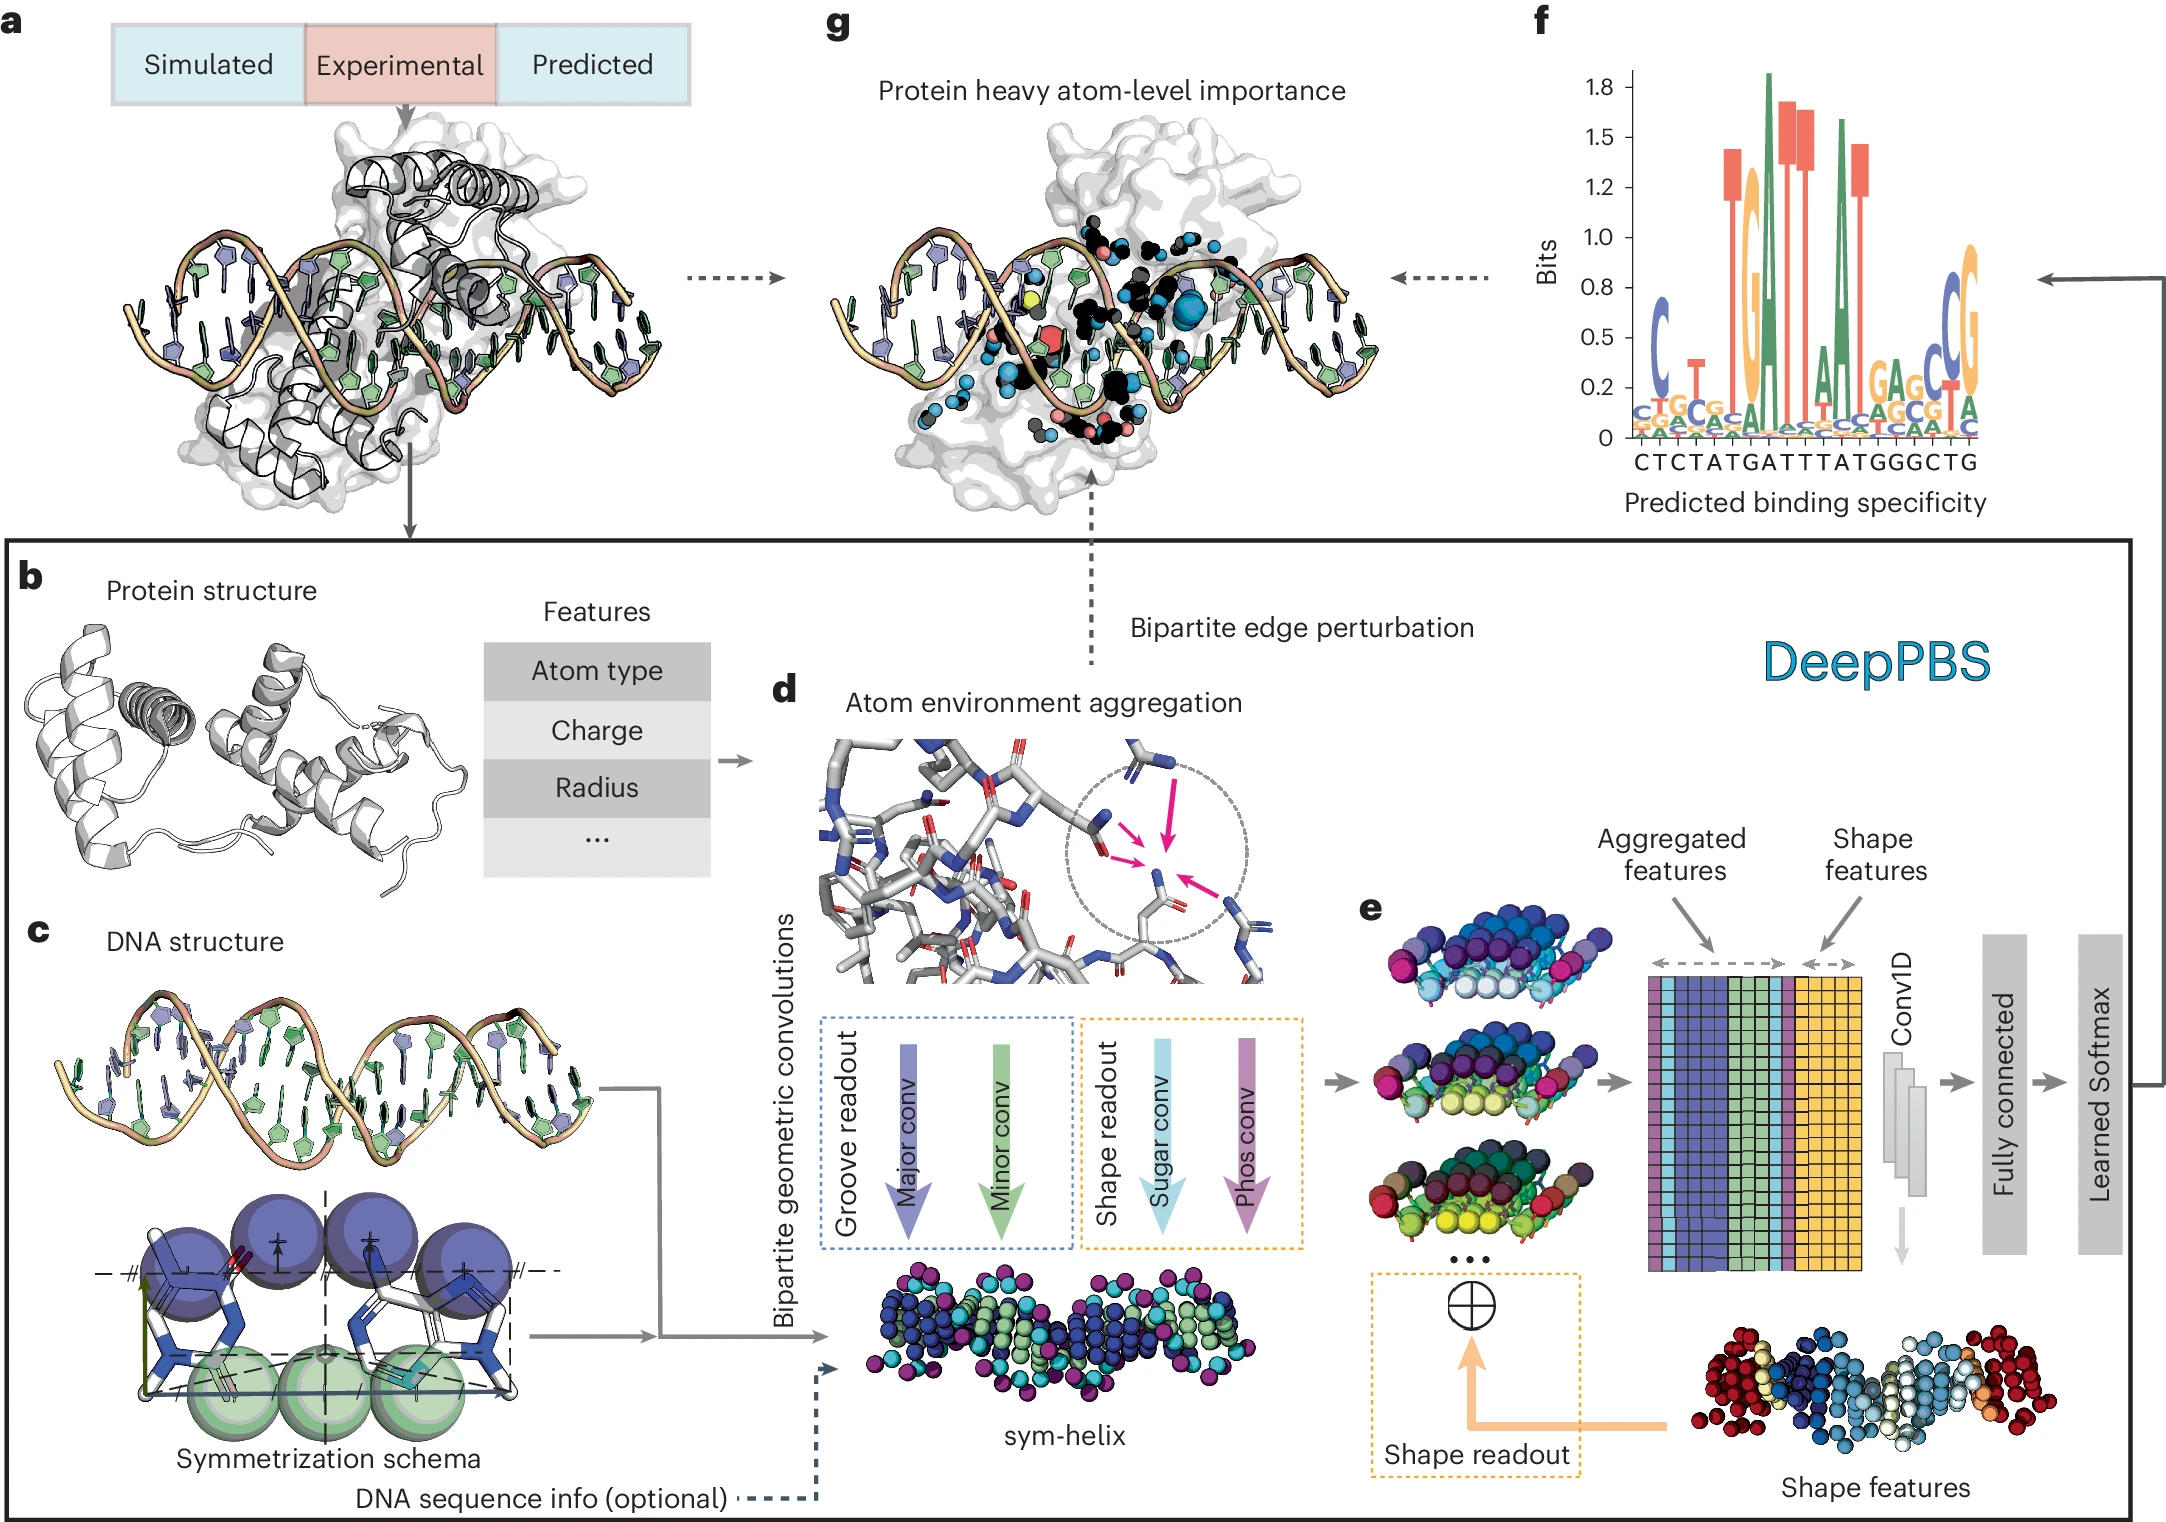
\includegraphics[width=0.8\paperwidth]{./pdna_figs/fig1.png}}
 % archetecture.png: 1149x508 px, 72dpi, 40.53x17.92 cm, bb=0 0 1149 508
        \caption[Computational cost of training RVAgene]{\textbf{Training RVAgene is reasonably scalable on CPU and even more so using hardware acceleration through GPU.} ({\bf A}) Time cost of training RVAgene for 100 epochs for datasets with varying number of genes and time points on CPU and GPU. ({\bf B}) Maximum memory utilized during training of the model on CPU an GPU for the cases in (A), inset plot: comparison of max memory used compared to DPGP for varying number of genes.}
  \label{fig:pdna1}
\end{figure}
\end{center}
\subsection{Representing Protein}
In our framework protein is viewed as a spatial graph $G^p = (V^p, X^p, E^p, N^p)$  where the
coordinates of the heavy atoms constitute the vertices $V^p$. For each vertex $v \in V^p$  we define
a set of features $X^p_v$ which include one hot encoded atom type, solvent accessible surface area
of the atom, charge, radius, circular variance and Atchley factors. The edges $E^p$ of the protein
graph  are determined by the covalent bonds i.e. if  vertices $u$ and $v$ have
a covalent bond between them then $(u,v) \in E^p$. The edges are unordered. Lastly to encode
directionality of protein side chains we encode a unit vector $N^p_v$ for each vertex $v$ computed by
averaging the directions of convalent bonds associated with each heavy atom. 
\subsection{Representing DNA}
Unlike the protein, a few important considerations need to be taken into account for representing
DNA in this framework. First, our model would see the structure of DNA in the input but shall predict a one
dimensional representation (a PWM), therefore in a purely engineering sense, it will be helpful to
have same number of features per basepair. Second, the input co-crystal DNA has a sequence, depending on
use cases we may or may not want our model to see this sequence, also since structure data is sparse
the  co-crystal sequence has a strong potential for overfitting if seen by the model in input.
Therefore, in general we want to symmetrize each base pair such that all the sequence information is
lost but global shape of the DNA structure is preserved.
With these points in mind, we come up with a coarse grained represntation of DNA
where we represent each basepair as 11 points, 2 points representing the Phosphate moeity on each
strand, 2 points represneting the Sugar moeity, 4 points in the major groove and 3 points in the minor
groove. The major and minor groove points are placed symmetrically in the basepair plane so that
they are devoid of any particular base identity but roughly correspond to the major and minor
groove chemical positions known \red{cite chiu. et. al. PNAS, 2023} to be used for base readout. Further
details about how these points are chosen are in the \red{supplementary, cite olson2001standard for
basepairframe}. Hence, the DNA structure is represented as $G^d = (V^d, X^d, N^d)$. $V^d$ represents
coordinates of the coarse grained points, $X^d$ represents point level DNA features which simply
include one hot encoded annotation about which of the 11 points it is in the coarse grained
base-pair representation. It should be noted that, if we desire we can add back the DNA sequence by
including base-pair specific chemical interaction features for each point to $X^d$ in the same manner as \red{cite
chiu. et. al.}. For each point $v \in X^d$ we also define an interaction vector $N^d_v$. These
vectors used are basically reference directions in base-pair frame and used to compute relative
orientation based features coupled with the vectors $N^p$ on the protein graph discussed further
ahead. In addition we also include 14 DNA shape features denoted as $X^s$ which are basepair level features, further
details in \red{supplementary}.
\subsection{DeepPBS}

\begin{center}
    \begin{figure}
    \makebox[\textwidth]{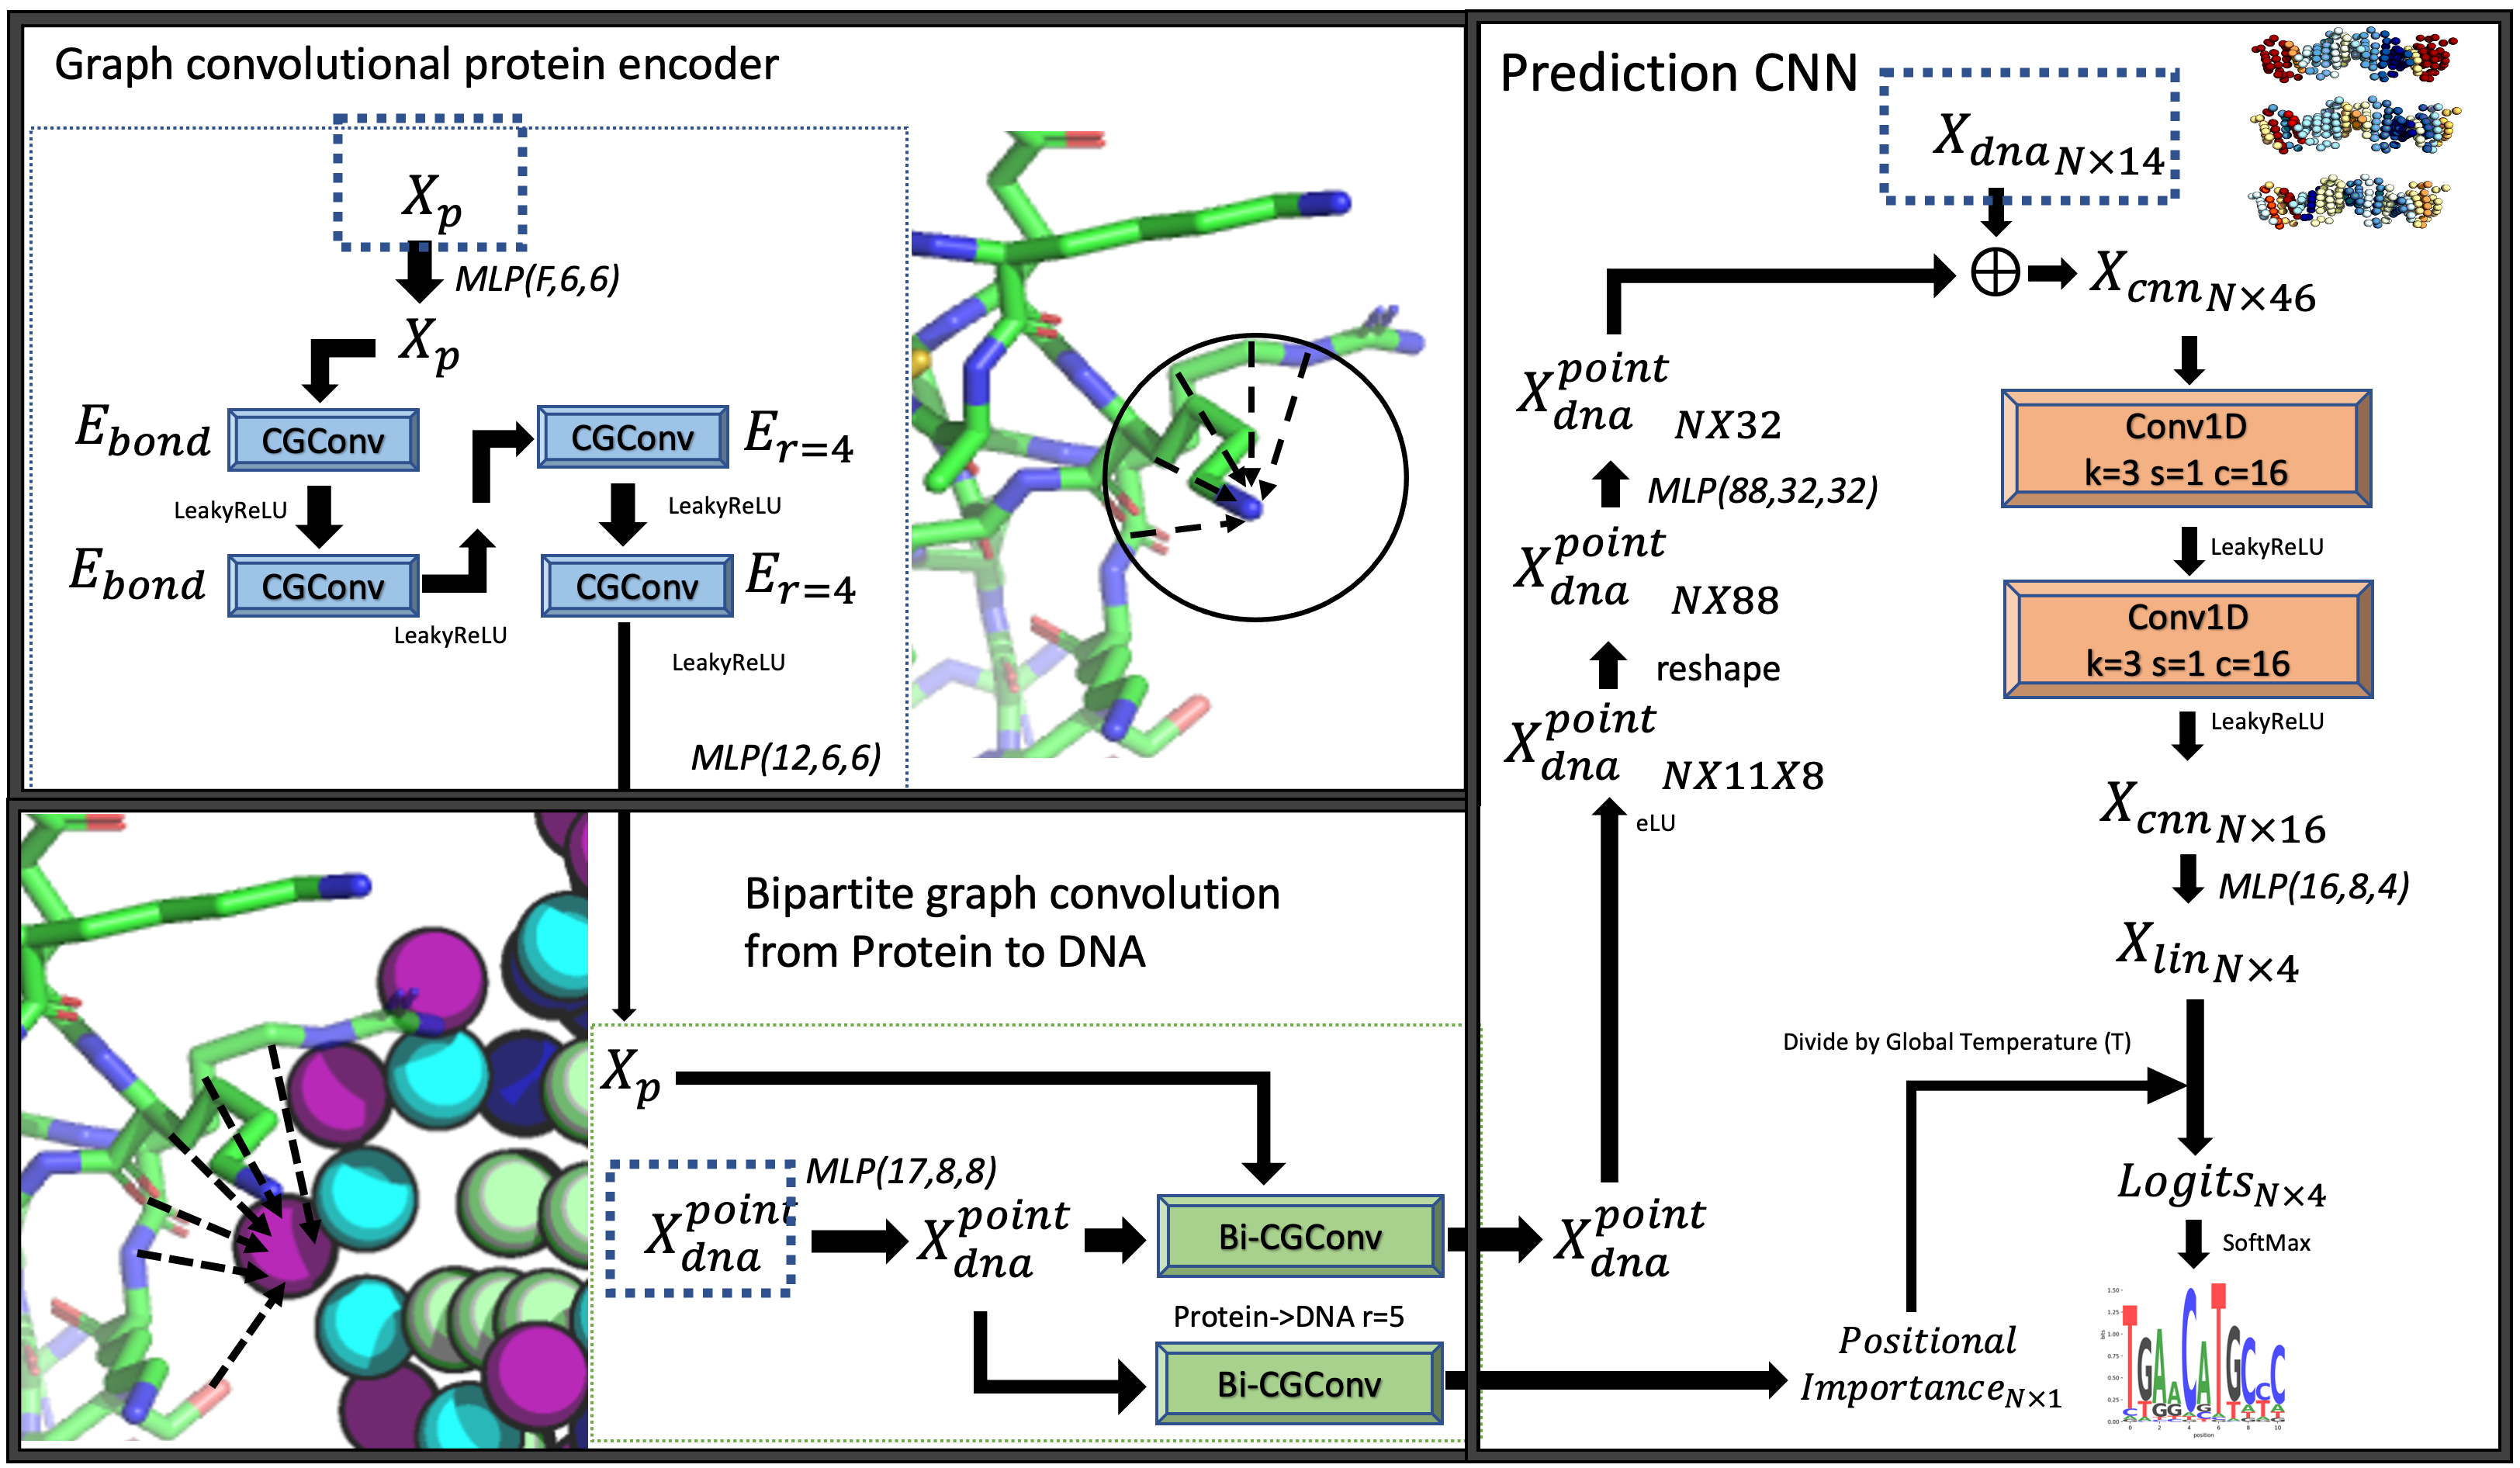
\includegraphics[width=0.8\paperwidth]{./pdna_figs/fig2.png}}
 % archetecture.png: 1149x508 px, 72dpi, 40.53x17.92 cm, bb=0 0 1149 508
        \caption[Computational cost of training RVAgene]{\textbf{Training RVAgene is reasonably scalable on CPU and even more so using hardware acceleration through GPU.} ({\bf A}) Time cost of training RVAgene for 100 epochs for datasets with varying number of genes and time points on CPU and GPU. ({\bf B}) Maximum memory utilized during training of the model on CPU an GPU for the cases in (A), inset plot: comparison of max memory used compared to DPGP for varying number of genes.}
  \label{fig:pdna2}
\end{figure}
\end{center}
\subsection{Evaluation Metrics}

